\documentclass[aspectratio=169]{beamer}
\input{000-preamble.tex}
%      ^^^^^^^^^^^^^^^^
% a preamble file.
% It might import stuff required for the theme, but I didn't try to figure out which ones

%%%%%%%%%%%%%%%%%%%%%%%%%%%%%%%%%%%%%%%%%%%%%%%%%%%%%%%%%%%%%%%%%%%%%%%%%%
% The theme
% see the files themselve to personalize it
\newcommand{\themedirectory}{./001-custom-theme/}
%                            ^^^^^^^^^^^^^^^^^^^
% the directory that holds the theme, because beamer is dumb, we need to redefine the `\usetheme'
% command (and it's derivitives).
% https://tex.stackexchange.com/a/435558/236175
\makeatletter
\def\beamer@calltheme#1#2#3{%
  \def\beamer@themelist{#2}
  \@for\beamer@themename:=\beamer@themelist\do
  {\usepackage[{#1}]{\themedirectory#3\beamer@themename}}}
\makeatother
\usetheme{secpriv}
% ^^^^^^^^^^^^^^^^ <- actually calls the theme
% Note that `secpriv` resets the `\usethem` command afteward

%%%%%%%%%%%%%%%%%%%%%%%%%%%%%%%%%%%%%%%%%%%%%%%%%%%%%%%%%%%%%%%%%%%%%%%%%%
\usepackage{minted, soul, multimedia}

\title{Computationally Sound Automated Protocol Verification}
\subtitle{Cryptovampire}
\date{\today}
\author{Simon \textbf{Jeanteur}}

\begin{document}

\begin{frame}[plain]
  \titlepage
\end{frame}
\begin{frame}
  This slide is required, otherwise the template breaks

  TODO: fix bugs with \LaTeX, newline on the titlepage often fail
\end{frame}

% \tableofcontents

\section{Introduction}

\begin{frame}
  \frametitle{Protocols}

  \hfill\pause
  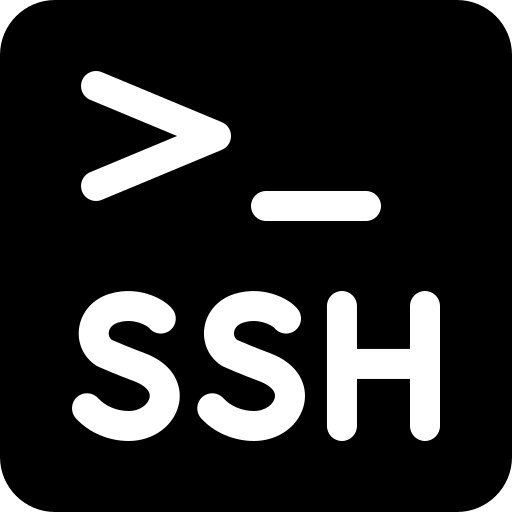
\includegraphics[width=.2\textwidth]{012-Assets/image5.png}
  \hfill\pause
  
\includegraphics[width=.2\textwidth]{012-Assets/image6.png}
  \hfill\pause
  
\includegraphics[width=.2\textwidth]{012-Assets/image8.png}
  \hfill

\end{frame}

\begin{frame}
  \frametitle{When cryptography is not enough}

  \begin{columns}
    \begin{column}{0.45\textwidth}
        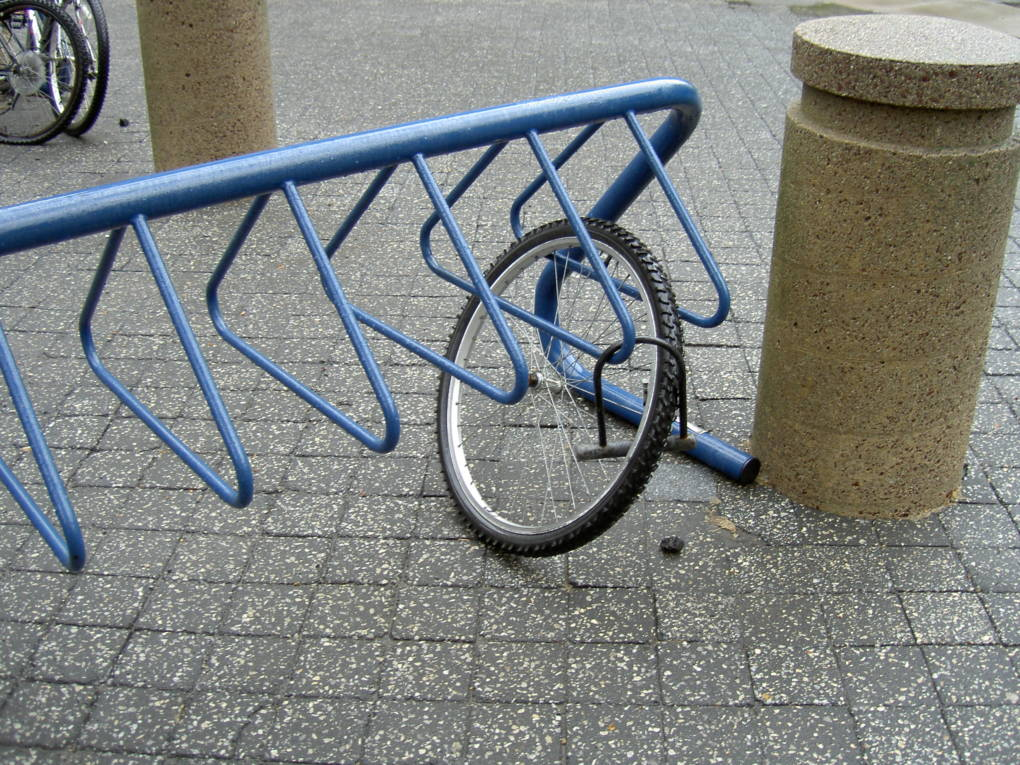
\includegraphics[width=\textwidth]{012-Assets/bike.jpg}
    \end{column}\centering
    \pause
    \begin{column}{.45\textwidth}
        % 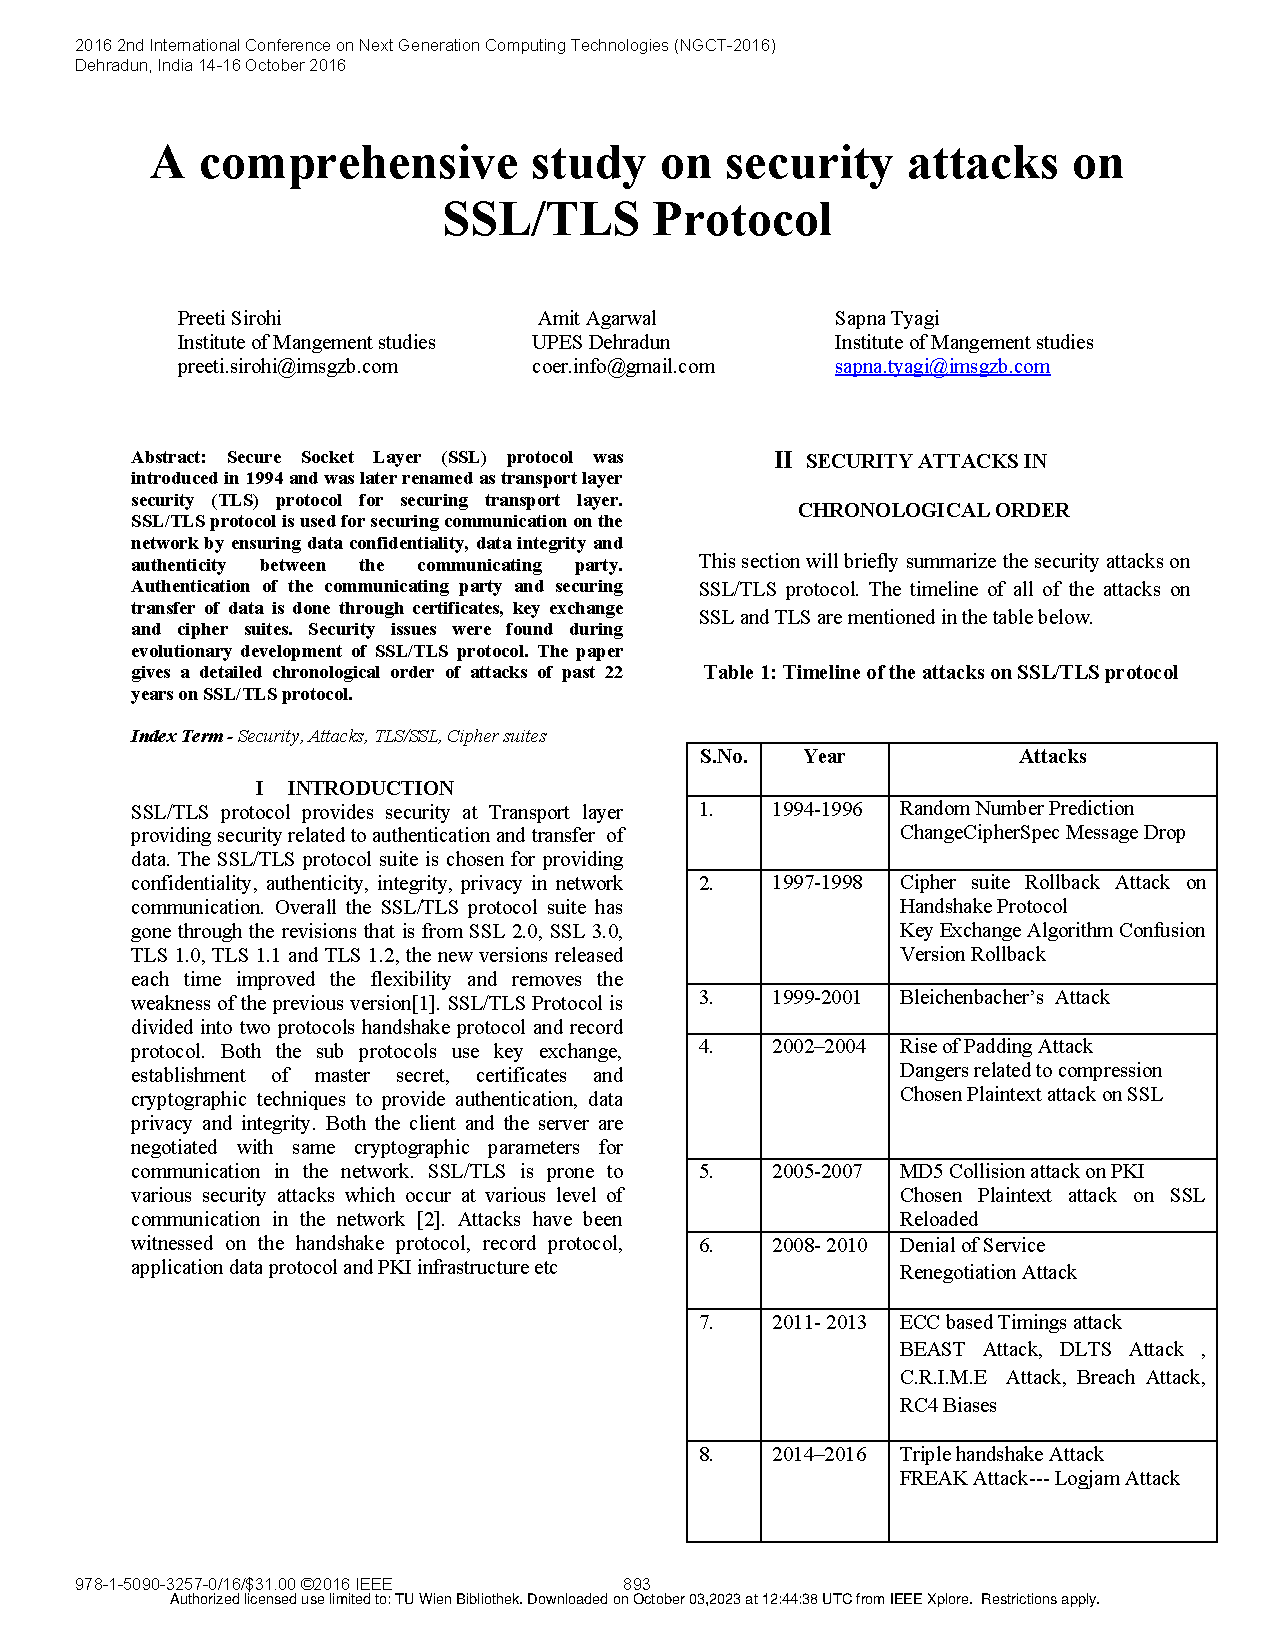
\includegraphics[width=.8\textwidth]{012-Assets/Sirohi et al. - 2016 - A comprehensive study on security attacks on SSLT.pdf}
      
        \begin{tikzpicture}[baseline=(paper1.north)]
          % First paper
          \node[fill=white, draw=black, rounded corners=2pt] (paper1) at (0,0) {
              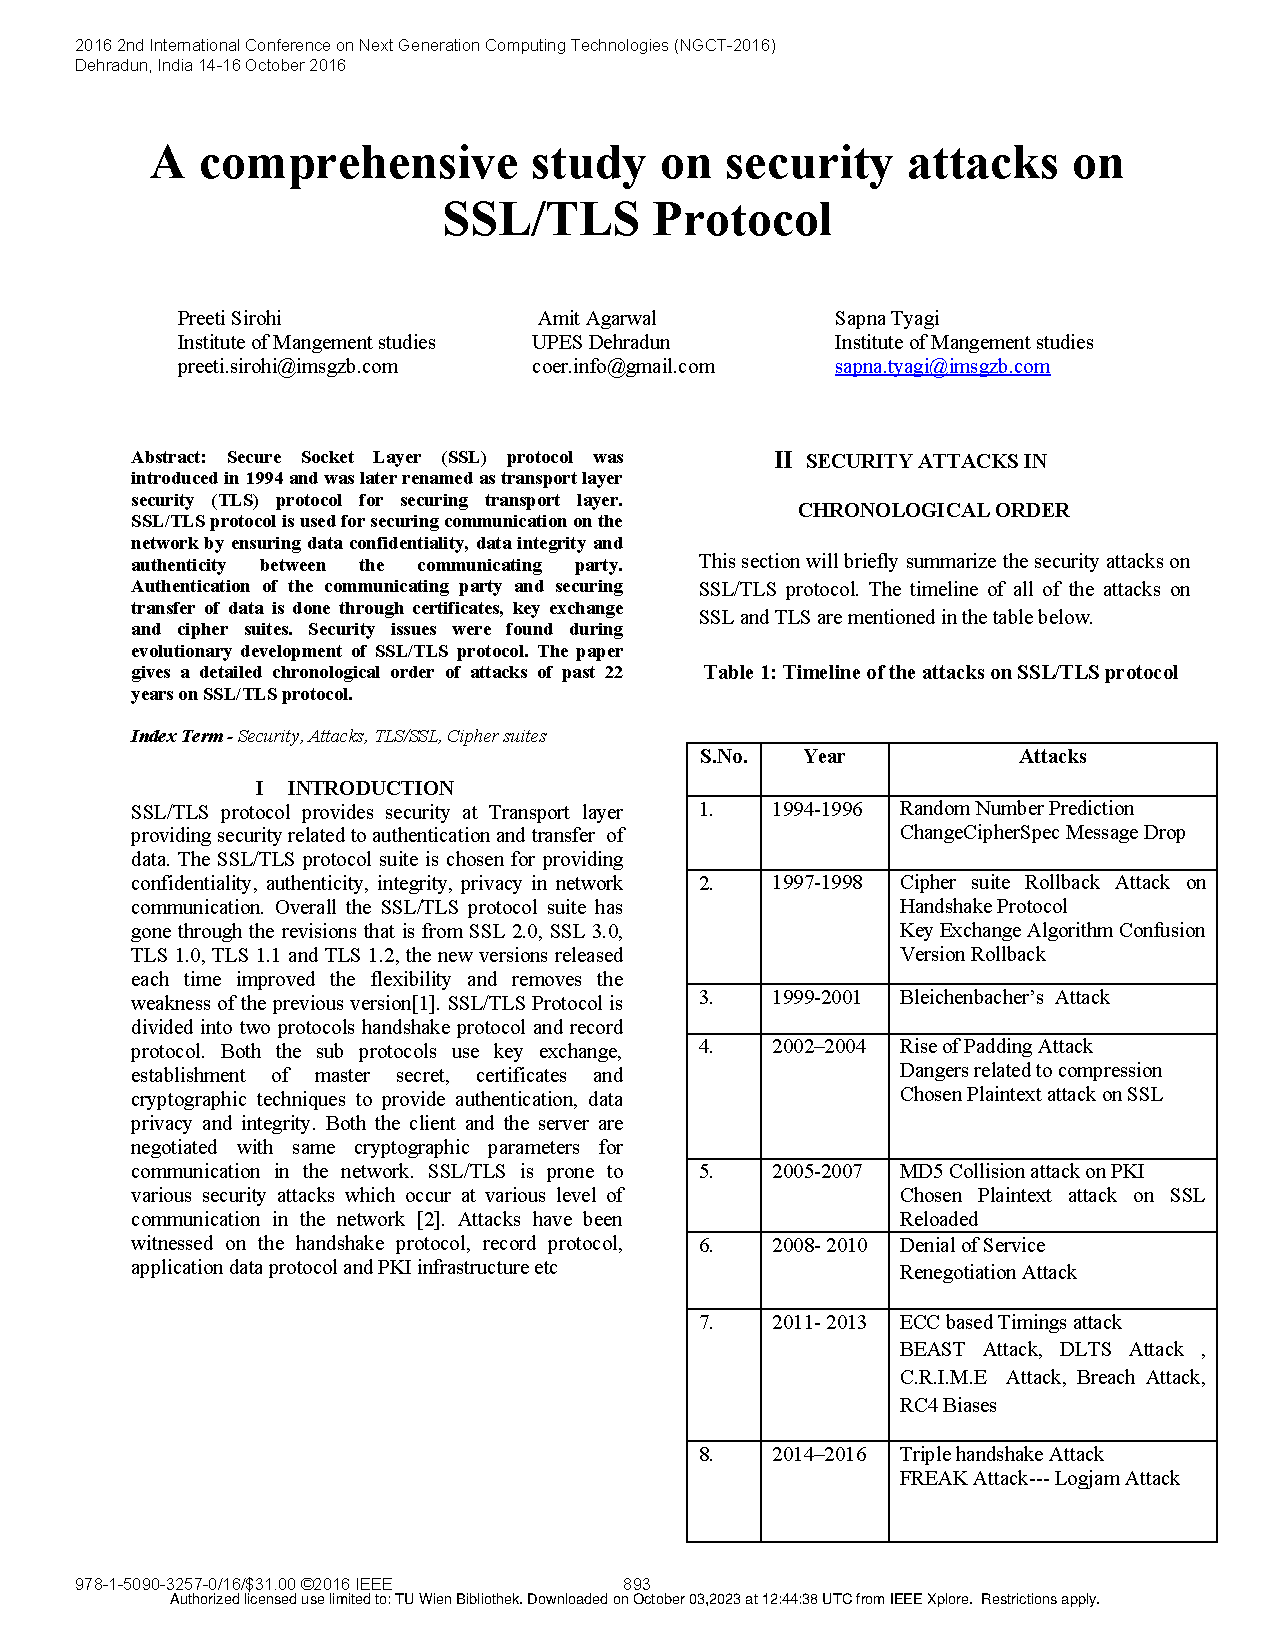
\includegraphics[width=0.8\textwidth]{012-Assets/Sirohi et al. - 2016 - A comprehensive study on security attacks on SSLT.pdf}
          };
          \pause
  
          % Second paper slightly offset and overlapping the first
          \node[fill=white, draw=black, rounded corners=2pt] (paper2) at (0.5, -0.5) {
              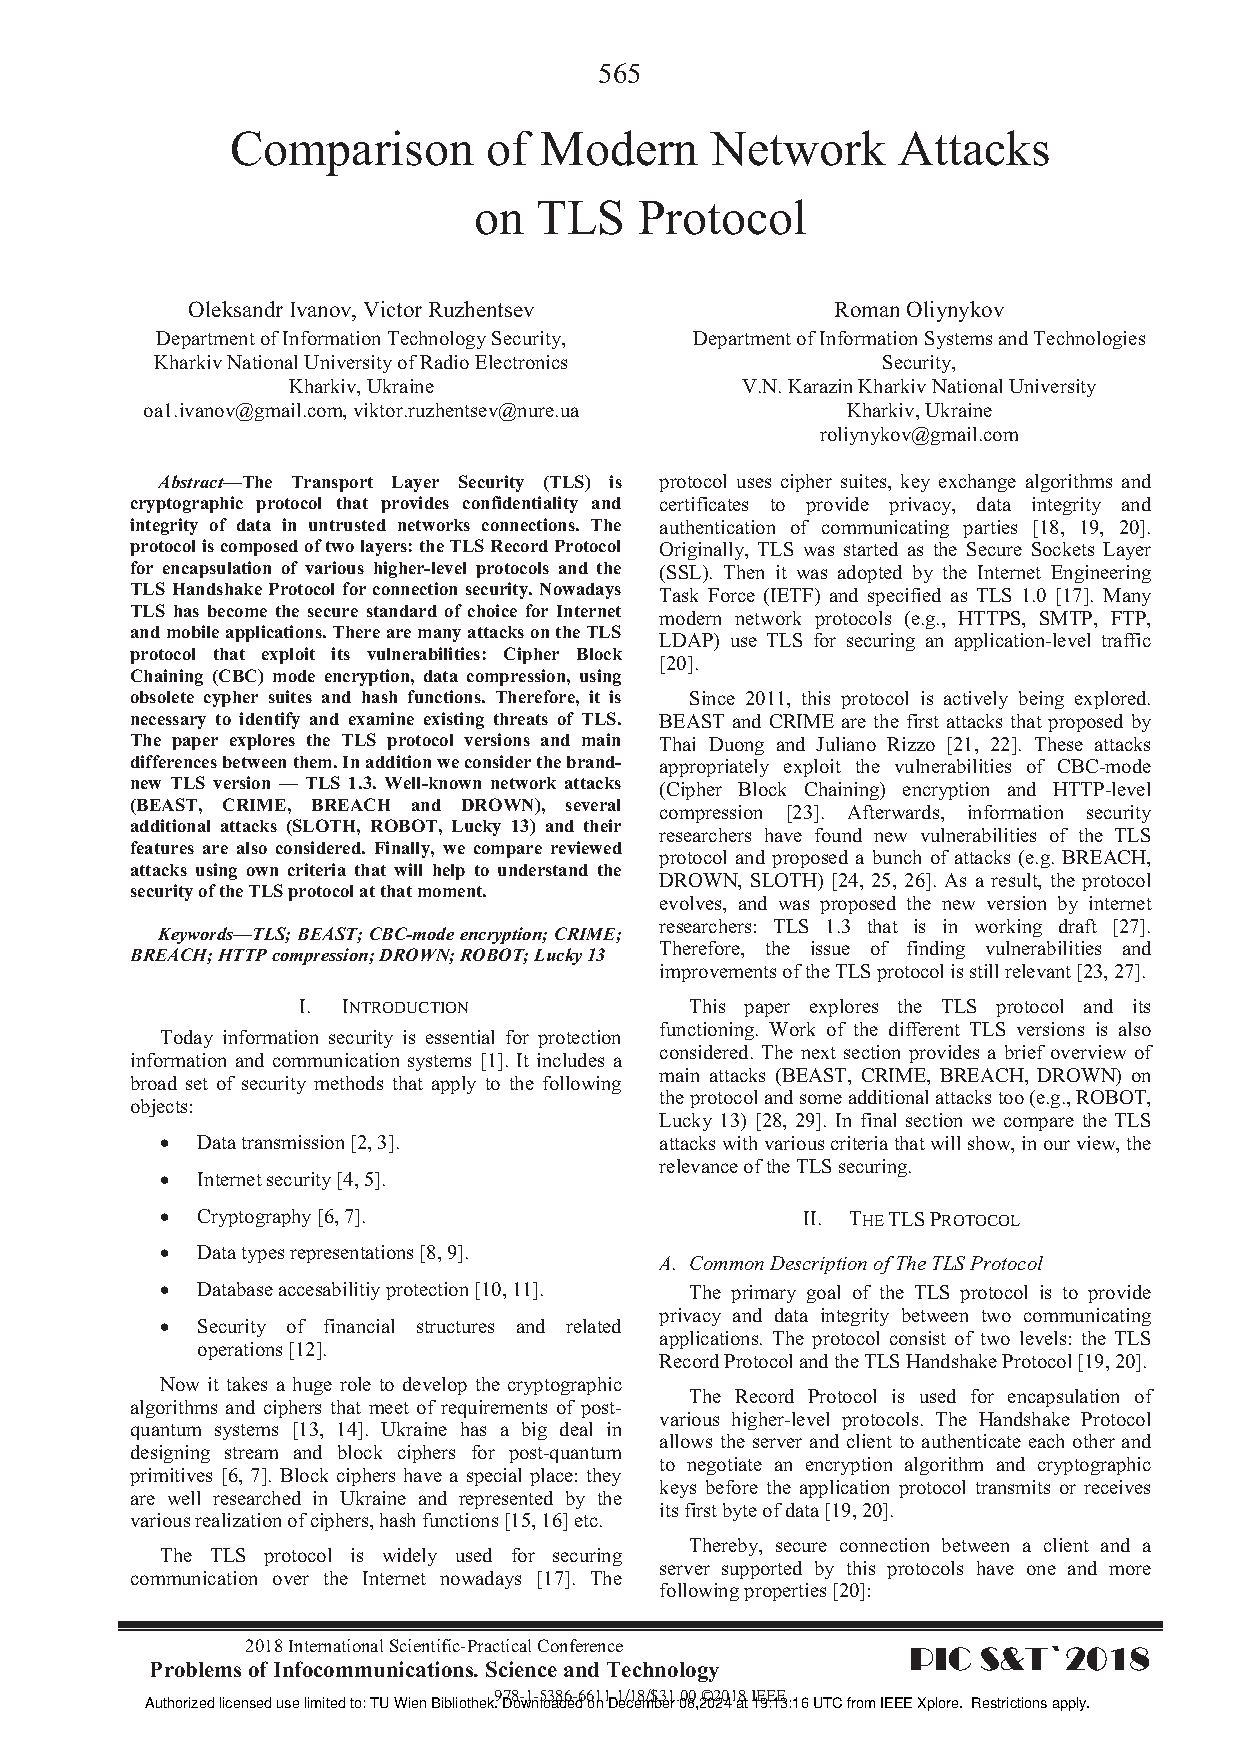
\includegraphics[width=0.8\textwidth]{012-Assets/Comparison_of_Modern_Network_Attacks_on_TLS_Protocol.pdf}
          };
      \end{tikzpicture}
    \end{column}
  \end{columns}
\end{frame}

\subsection{What is a \enquote{secure} protocol?}

\begin{frame}
  \frametitle{Threat Model \& Propreties}

  \begin{columns}
    \begin{column}{0.45\textwidth}
      \underline{\textbf{Properties}}:\pause
      \begin{enumerate}
        \item \emph{Trace} propreties: \pause\begin{itemize}
          \item Is $k$ kept secret?\pause
          \item Are we sure that \textit{this} part of the protocol takes place before \textit{that} part?\pause
        \end{itemize}
        \item \emph{Indistinguishability} / Observationnal equivalence: \pause\begin{itemize}
          \item Can the attacker tell protocol $1$ appart from protocol $2$?
        \end{itemize}
      \end{enumerate}
    \end{column}
    \begin{column}{0.5\textwidth}\pause
      Who is the attacker?
      \begin{itemize}\pause
        \item No perfect security $\Rightarrow$ probabilitics security\pause
        \item Polynomial attacker
      \end{itemize}\pause
      \hrule

      Given keys of size $\eta$.\pause

      \underline{Trace}: given a proprety $P$,
      \[
        \boxed{\mathbb{P}\left( \AAA, \neg P \right) = \mnegl\left( \eta \right)}\pause = o\left( \eta^{-c} \right), c\in \mathbb{Z}
      \]\pause
      \underline{equivalence}: Given protocol $P_1$, $P_2$
      \[
        \boxed{\left| \mathbb{P}\left( \AAA\left( P_1 \right)=1 \right)-\mathbb{P}\left( \AAA\left( P_2 \right)=1 \right)\right| = \mnegl\left( \eta \right)}
      \]
    \end{column}
  \end{columns}
  

\end{frame}

\section{CCSA}
\subsection{BC Logic}
\begin{frame}
  \frametitle{BC Logic -- Syntax}

  \[
      \boxed{t:= x \gsep \n \gsep f\left( t_1, \dots, t_n \right) \gsep \matt\left( t \right)}
  \]  
  where $t\in \mathcal{X}_\mathrm{bc}$, $f\in\mfunctionsbc$ (finite), $\n\in\mnoncesbc$ (finite)

\end{frame}

\begin{frame}
  \frametitle{BC Logic -- Semantics}

  We want an evaluation function $\mevalbc{\cdot}$ such that:
  \begin{itemize}
    \item Nonce are random\pause, independent \pause and of the right length ($\eta$)\pause
    \item Deterministic function comppute the expected fonction\pause
    \item The attaker is a PPTM
  \end{itemize}\pause

  \Rightarrow make $\mevalbc{\cdot}$ a familly random variable indexed by $\eta$
  \pause

  Let $\rho =\left( \rho_h, \rho_\AAA \right)$ be a pair of random tapes:
  \hfill {\footnotesize $t:= x \gsep \n \gsep f\left( \vec{t} \right) \gsep \matt\left( t \right)$}
  \begin{align*}
    \mevalbc{\n}\left( 1^\eta, \rho \right)&:= \text{slice of length $\eta$ of ${\color{tublue}\rho_h}$}\\
    \mevalbc{f\left( t_1, \dots, t_n \right)}\left( 1^\eta, \rho \right)&:= \mathbb{M}\left( f \right)\left( 1^\eta; \mevalbc{t_1}\left( 1^\eta, \rho \right), \dots,  \mevalbc{t_n}\left( 1^\eta, \rho \right) \right)\\
    \mevalbc{\matt\left( t \right)}&:= \matt_\mathbb{M}\left( 1^\eta, {\color{tumagenta} \rho_\AAA}; \mevalbc{t}\left(1^\eta, \rho \right) \right)
  \end{align*}
\end{frame}

\begin{frame}
  \frametitle{BC Logic -- Properties}

  Let $u$, $v$ and $P$ be BC terms, we define

  \begin{itemize}
    \item \underline{Trace}:
  \[\boxed{\validp P} \text{ iff. }\mprob\left( \mevalbc{P}\left( 1^\eta, \rho \right) \neq 1 \right)=\mnegl\left( \eta \right)\]
  e.g.: $\matt\left( \text{frame} \right)\neq \mk$, $\text{Begin} < \text{End}$, \dots...
%
    \item \underline{Indistinguishability}:
  \[\boxed{u \sim v} \text{ iff. }\left|\mprob\left( \AAA\left( \mevalbc{P}\left( 1^\eta, \rho \right) \right) = 1 \right) - \mprob\left( \AAA\left( \mevalbc{v}\left( 1^\eta, \rho \right) \right) = 1 \right)\right|=\mnegl\left( \eta \right)\]
  e.g.: $P[\mk]~P[0]$
  \end{itemize}
\end{frame}

\subsection{Computationnally Complete Symbolic Attacker}

\begin{frame}
  \frametitle{Uninterpreted symbolic logic}

  We can rebuild a logic using the symbols in $f\in\mfunctionsbc$:
  \begin{itemize}
    \item e.g.: $ \beq $, $\bwedge$, $\mifthenelse{\_}{\_}{\_}$,\dots
  \end{itemize}

\end{frame}

\begin{frame}
  \frametitle{Rules: an example}\pause

  \begin{mtheoremenv}{No Guessing Theorem}{}
    It is almost impossible to guess a nonce.
  \end{mtheoremenv}\pause

  \[
    \frac{\text{\only<3>{$\n$ appears in $t$}} \only<4>{\n\sqsubseteq t}}{\validp \n \beq t}
  \]

\end{frame}

\begin{frame}
  \frametitle{Rules: General form}

  \[
    \text{Classical Logic rules} +
    \frac{\color{tumagenta} \text{symbolic fact}}{\color{tublue} \text{evaluation fact}}
  \] \pause

  This looks fairly automatable as:\pause
  \begin{itemize}
    \item {\color{tublue} evaluation fact}: Theory of equality\pause
    \item {\color{tumagenta} symbolic fact}: Theory of datatypes
  \end{itemize}

\end{frame}

\section{CryptoVampire}

\begin{frame}
  \frametitle{Cryptovampire}

  An automated protcol verifier for trace properties using the CCSA: [SP23]
  % 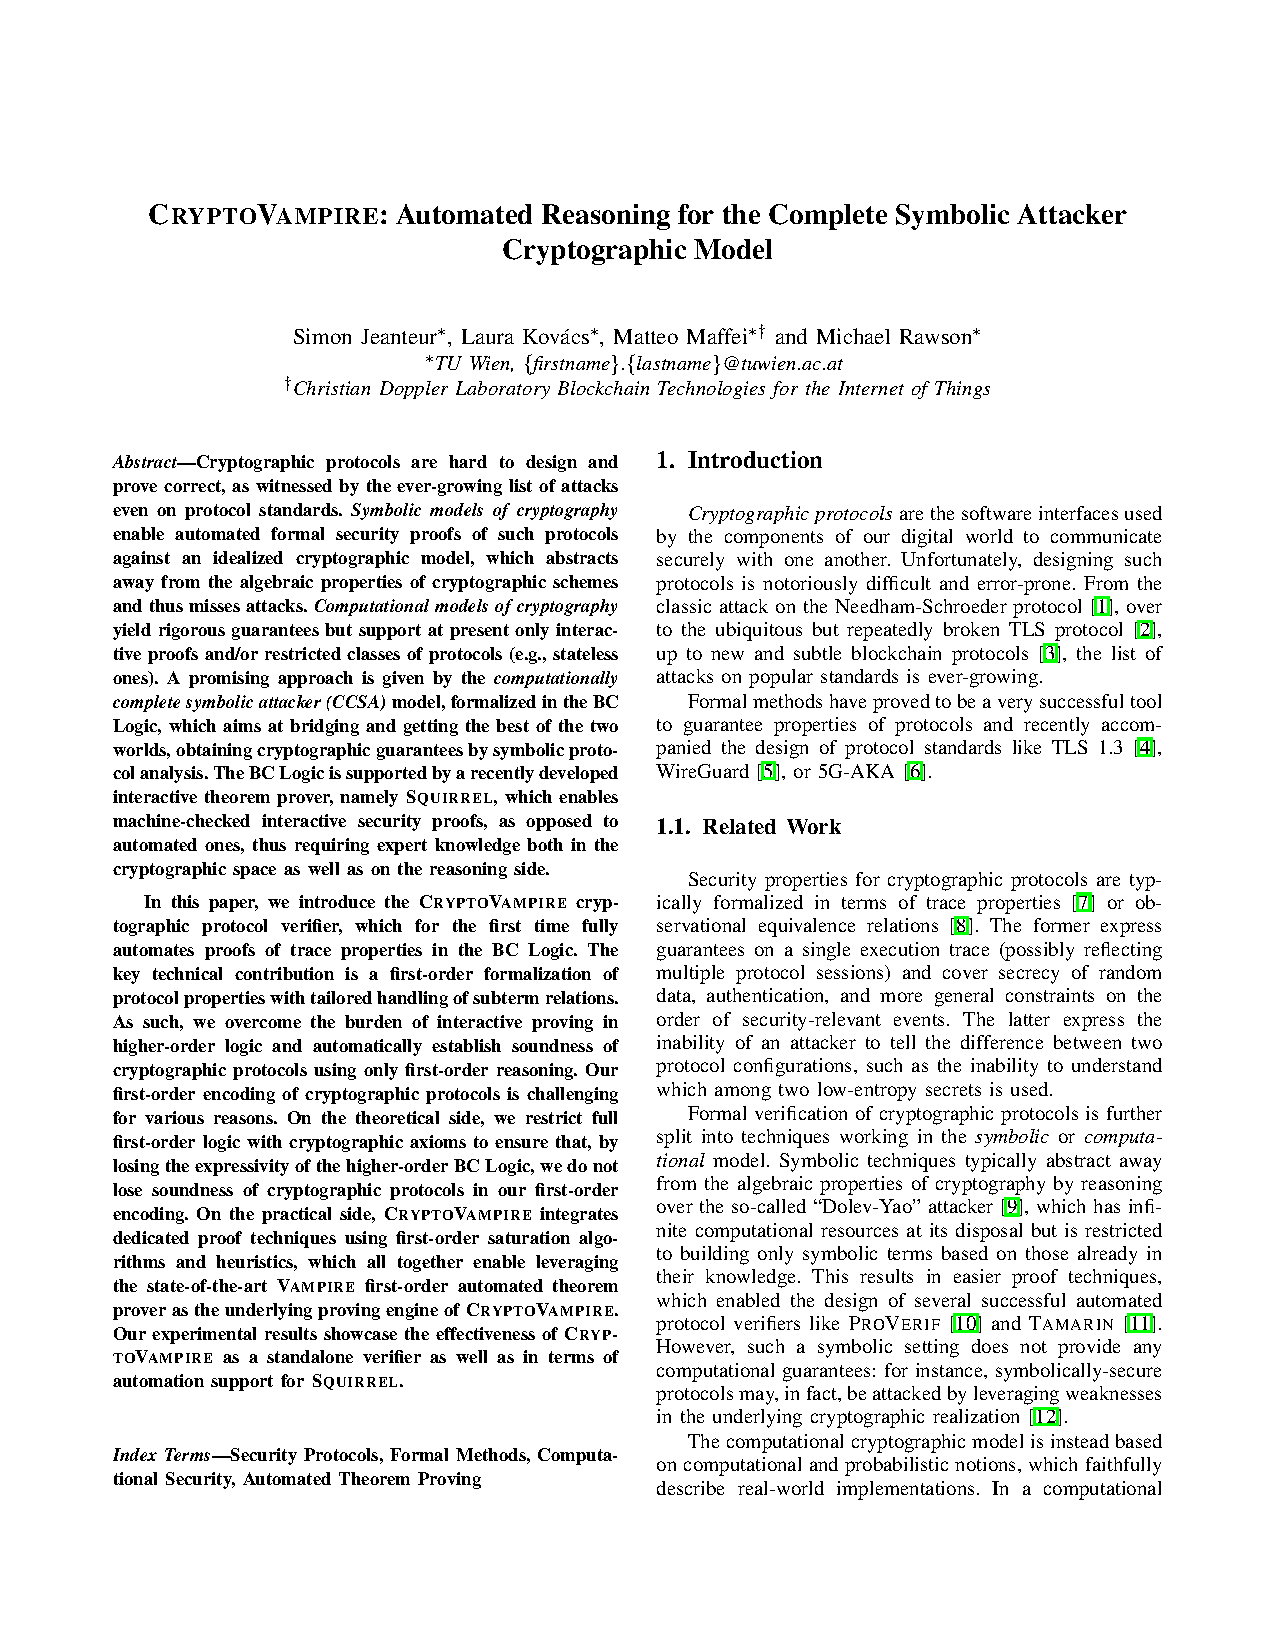
\includegraphics[width=.8\textwidth]{012-Assets/cryptovampire.pdf}
  \centering
  \begin{tikzpicture}[baseline=(paper1.north)]
      % First paper
      \node[fill=white, draw=black, rounded corners=2pt] (paper1) at (0,0) {
          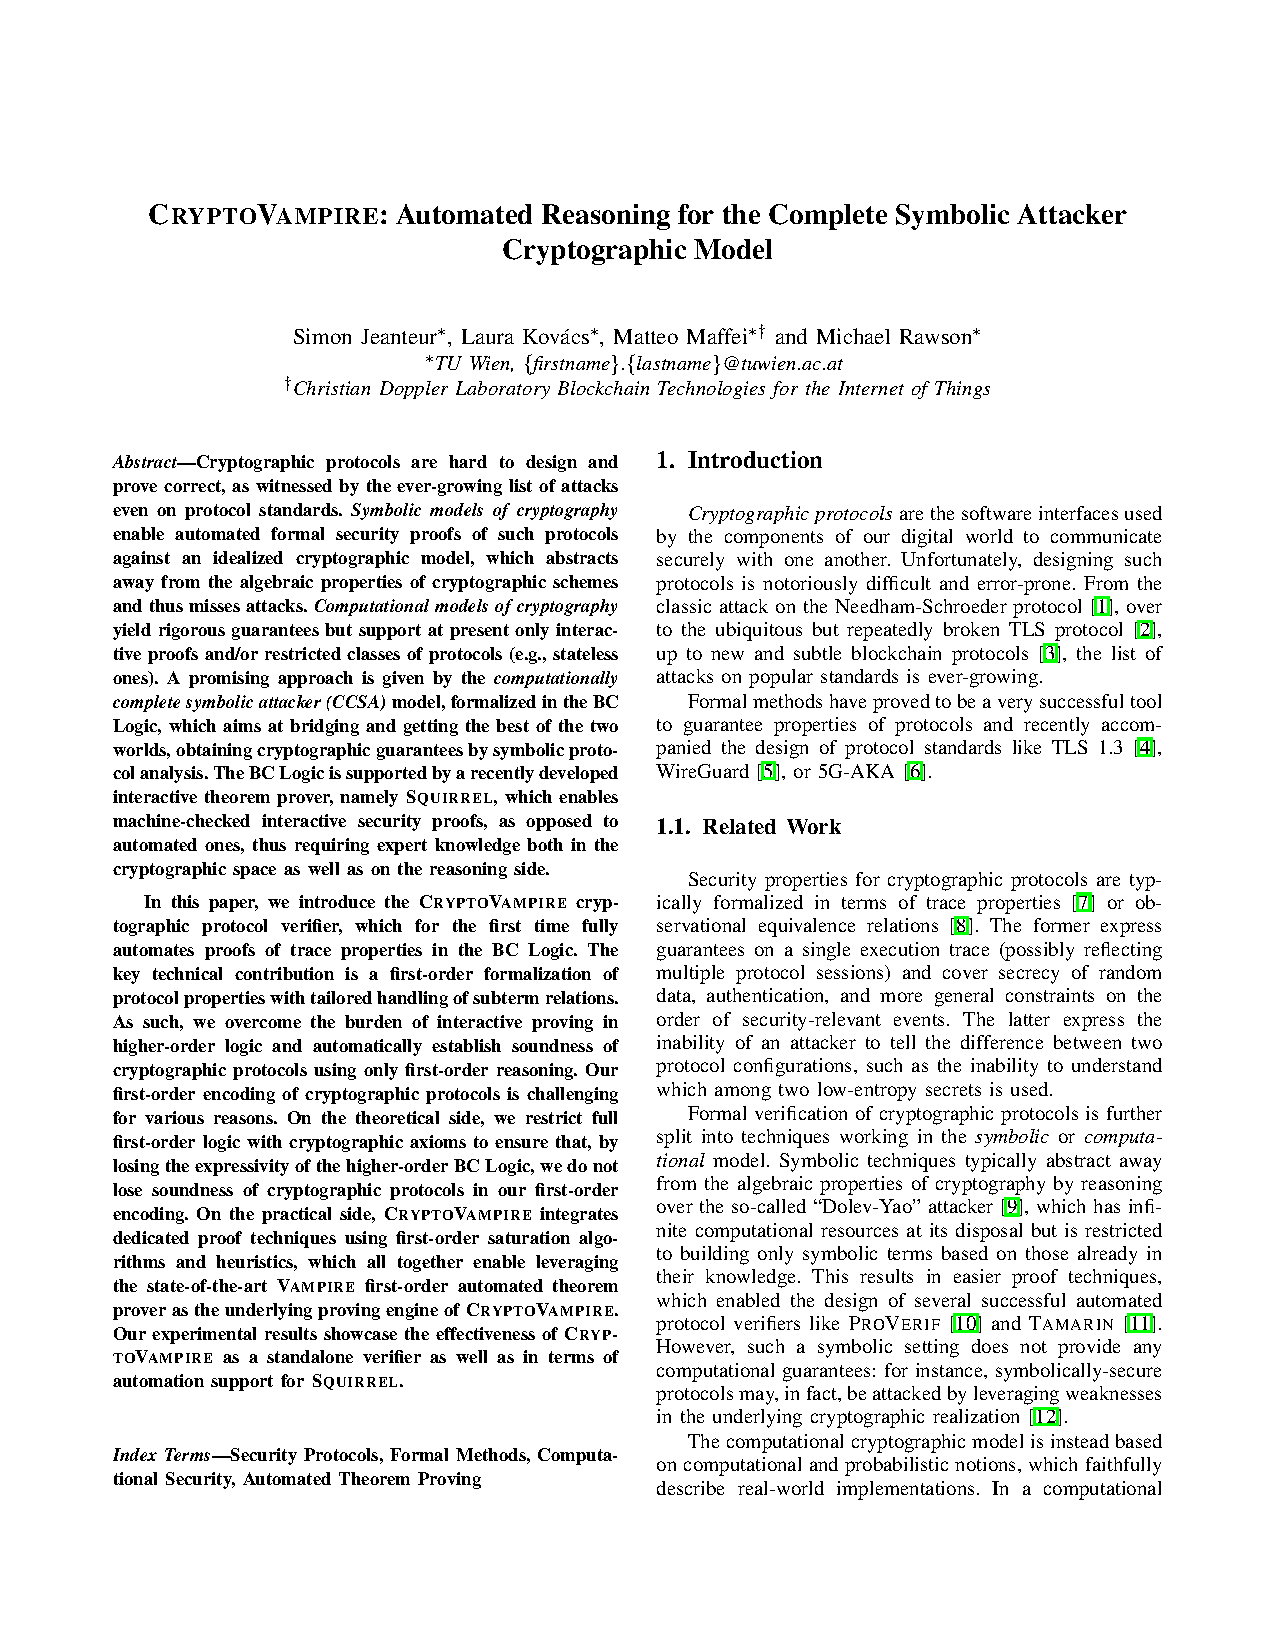
\includegraphics[width=0.8\textwidth]{012-Assets/cryptovampire.pdf}
      };
  \end{tikzpicture}
\end{frame}

\begin{frame}
  \frametitle{The dream}
  \pause

  \begin{enumerate}
    \item Encode the CCSA in FOL\pause
    \item Encode the protocol in FOL\pause
    \item Dump everything into a FOL theorem prover \pause {\RajdhaniRg(e.g., vampire)}\pause
    \item ???\pause
    \item Profit
  \end{enumerate}

\end{frame}

\begin{frame}
  \frametitle{The reality}

  \begin{enumerate}
    \item \st{Encode the CCSA in FOL}
    \item Encode the protocol in FOL
    \item Dump everything into a FOL theorem prover {\RajdhaniRg(e.g., vampire)}
    \item \st{???}
    \item Profit
  \end{enumerate}

\end{frame}

\subsection{Solving problems}
\begin{frame}
  \frametitle{Subterms \& Equality}

  \begin{columns}
    \begin{column}{.45\textwidth}
      Remember:
      \[
        \frac{\color{tumagenta}\n\sqsubseteq t}{\validp \n \beq t}
      \]\pause
      So
      \[
        \n = t \Rightarrow \n\sqsubseteq t
      \]\pause
      \emph{Inconsistent.}
    \end{column}

    \begin{column}{.45\textwidth}\pause

      Consider:
      \begin{itemize}
        \item $\n \sqsubseteq \mk$ ? \pause \emph{No}\pause, but...
        \item $\mk \beq \pi_1\left( \left< \mk, \n\right> \right)$\pause
        \item but also $\n \sqsubseteq \pi_1\left( \left< \mk, \n\right> \right)$
        \item thus $\n \sqsubseteq \mk$ \dots
      \end{itemize}
    \end{column}
  \end{columns}\pause\hrule
    We need to split $\sqsubseteq$ from $\beq$:
    \begin{enumerate}
      \item Within the logic \pause (sound and complete but inefficient) \pause
      \item Within the decision procedure \pause (sound and efficient but incomplete)
    \end{enumerate}\pause
    We define the axioms using {\color{tublue}1.}, we optimise using {\color{tumagenta} 2.}.
\end{frame}

\begin{frame}
  \frametitle{Option 2: Preprocessing}

  Given an axiom
  \[
      \frac{\color{tumagenta} \mathrm{symb}\left[ \vec t \right]}{\color{tublue} \mathrm{eval}\left[ \vec t \right]}
  \] \pause

  \begin{itemize}
    \item find all $\mathrm{eval}\left[ \vec t_1 \right]$, $\mathrm{eval}\left[ \vec t_2 \right]$, \dots\ in the protocol, queries, \dots \pause
    \item preprocess $\mathrm{symb}\left[ \vec t_1 \right]$, $\mathrm{symb}\left[ \vec t_2 \right]$, \dots\ to the point they to depends on \textit{symbolic} reasoning anymore\pause
    \item reintroduce axioms
  \end{itemize}

\end{frame}

\begin{frame}
  \frametitle{Automated interataction}

  It is possible to learn from a failed run:
  \pause

  \begin{enumerate}
    \item Run the FOL theorem prover a first time\pause
    \item Gather all the synthethised terms\pause
    \item Look for new axiom instances in thoses\pause
    \item Add the new instance and go back to step 1
  \end{enumerate}

\end{frame}

\begin{frame}
  \frametitle{Lifting to first order}

  Let's reuse the Non-Guessing theorem:
  \[
    \frac{\n\sqsubseteq t}{\validp \n \beq t}
  \]\pause

  Converted to propositionnal logic, we get:
  \[
    \validp \meval{\n} = \meval{t} \Rightarrow \n \sqsubseteq t
  \]\pause

  This should hold \emph{for all} $t$, hence we'd like to add:
  \[
    \validp \forall t, \meval{\n} = \meval{t} \Rightarrow \n \sqsubseteq t
  \]\pause
\end{frame}

\begin{frame}
  \frametitle{Lifting to first order}

  We need a semantic for quantifiers:

  \[
    \mevalbc{\forall m, P\left[ m \right]}\left( 1^\eta, \rho \right) =\pause \begin{cases}
      1 &\text{if for all term $m$, } \mevalbc{P\left[ m \right]}\left( 1^\eta, \rho \right) = 0\pause\\
      0 & \text{otherwise}
    \end{cases}
  \]\pause
  \[
    \mevalbc{\exists m, P\left[ m \right]}\left( 1^\eta, \rho \right) = \begin{cases}
      1 &\text{if we can find a $m$, } \mevalbc{P\left[ m \right]}\left( 1^\eta, \rho \right) = 0\\
      0 & \text{otherwise}
    \end{cases}
  \]  

\end{frame}


\begin{frame}
  \frametitle{Counter example to classical semantics}

  \begin{columns}
    \begin{column}{0.37\textwidth}
      \begin{block}{{\color{tugreen} True} statement}
        For all $m$,
        \vspace*{-1mm}\[
          \validp \meval{\mk \beq m}\Rightarrow \mk \sqsubseteq m
        \]
      \end{block}\pause
    \end{column}

    \begin{column}{0.55\textwidth}
      \begin{block}{{\color{tumagenta} False} statement}
        \[
          \validp \forall m. \meval{\mk \beq m}\Rightarrow \mk \sqsubseteq m
        \]
      \end{block}
    \end{column}
  \end{columns}\pause
  \vspace*{3mm}
  Indeed, for any $\eta$ and $\rho$, consider

  \begin{columns}
    \begin{column}{0.37\textwidth}
      \[
        \mathsf{n}^{\eta,\rho}_{\mk}\coloneqq \mathsf{succ}^{\bcint{\mk}{\eta}{\rho}}\left( 0 \right)
      \]\pause
    \end{column}
    \begin{column}{0.55\textwidth}
      We have
      \begin{itemize}[<+->]
        \item $ \bcint{\mk}{\eta}{\rho} = \bcint{\mathsf{n}^{\eta,\rho}_{\n}}{\eta}{\rho}$
        \item $ \bcint{\meval{\mk \beq \mathsf{n}^{\eta,\rho}_{\mk}}\Rightarrow \mk \sqsubseteq \mathsf{n}^{\eta,\rho}_{\mk}}{\eta}{\rho} = 0 $
      \end{itemize}
    \end{column}
  \end{columns}

  % Indeed, for any $\eta$ and $\rho$, writting $\text{succ}^{\mdice}\left( 0 \right) \coloneqq \mathsf{succ}^{\bcint{\mdice}{\eta}{\rho}}\left( 0 \right)$ we have
  % \[
  %   \bcint{\mdice}{\eta}{\rho} = \bcint{\text{succ}^{\mdice}\left( 0 \right)}{\eta}{\rho}
  % \]
  % thus
  % \[
  %   \bcint{\meval{\mdice \beq \text{succ}^{\mdice}\left( 0 \right)}\Rightarrow \mdice \sqsubseteq \text{succ}^{\mdice}\left( 0 \right)}{\eta}{\rho} = 0
  % \]

\end{frame}

\begin{frame}
  \frametitle{Recovering FOL}

  \begin{theorem}
    For any formula $\varphi$ and term $t$, {\bfseries if}\pause
    \begin{enumerate}[<+->]
      \item\label{item:th:main:1} $\varphi$ is well formed;
      \item\label{item:th:main:2} for all $\vecvb$, $\validp \msubstit{\varphi}{\vecu}{\vecvb}$;
      \item\label{item:th:main:3} $\left( \forall\vecu.\ \varphi \right)\Rightarrow \meval{t}$ is valid in \emph{FOL};
    \end{enumerate}\pause
    {\bfseries then} $\validp \meval{t}$.
  \end{theorem}\pause

  We manually verify that all axioms verify \eqref{item:th:main:1} and \eqref{item:th:main:2} and use a theorem prover for \eqref{item:th:main:3}.

\end{frame}

% \begin{frame}
%   \frametitle{<title>}

  


\begin{frame}
  \frametitle{The new reality}\pause

  \begin{enumerate}
    \item Encode the CCSA in FOL \pause {\RajdhaniRg (using the theorem)}
    \item Encode the protocol in FOL\pause
    \item Dump everything into a FOL theorem prover {\RajdhaniRg (e.g., vampire)}\pause
    \item pray / use automated interaction\pause
    \item Profit
  \end{enumerate}

\end{frame}


% \section{Beyond CryptoVampire}

% \begin{frame}
%   \frametitle{Future work: Indistinguishability}

%     \movie[width=.4\textwidth,autostart,loop]{placeholder}{012-Assets/out.mp4}
% %     % \includegraphics[width=.8\textwidth]{012-Assets/output.gif}

% \end{frame}

















%%%%%%%%%%%%%%%%%%%%%%%%%%%%%%%%%%%%%%%%%%%%%%%%%%%%%%%%%%%%%%%%%
%%%%%%%%%%%%%%%%%%%%%%%%%%%%%%%%%%%%%%%%%%%%%%%%%%%%%%%%%%%%%%%%%
%%%%%%%%%%%%%%%%%%%%%%%%%%%%%%%%%%%%%%%%%%%%%%%%%%%%%%%%%%%%%%%%%
%%%%%%%%%%%%%%%%%%%%%%%%%%%%%%%%%%%%%%%%%%%%%%%%%%%%%%%%%%%%%%%%%
%%%%%%%%%%%%%%%%%%%%%%%%%%%%%%%%%%%%%%%%%%%%%%%%%%%%%%%%%%%%%%%%%
%%%%%%%%%%%%%%%%%%%%%%%%%%%%%%%%%%%%%%%%%%%%%%%%%%%%%%%%%%%%%%%%%

% \end{frame}

\section{Thank You!}


\section[Wait! What's a protocol in you setting?]{Protocol}

\begin{frame}
  \frametitle{Step \& Trace}

  A protocol is split in atomic \emph{steps}.\pause
  % \begin{block}{step}
  % \end{block}
  \begin{mdefenv}{Step}{}
    A \emph{step} is an atomic input/output guarded by a condition.
  \end{mdefenv}
  \pause

  We then verify the protocol over \emph{all}* orderings/interleaving/\emph{trace} of those steps.

\end{frame}

\begin{frame}
  \frametitle{Example}
  \begin{columns}
    \begin{column}{0.35\textwidth}


      Let's reuse the opening example:
      \begin{center}
        \begin{tikzpicture}
          \node at (3.2,0) (B) {\huge\emoji{man}};
          \node at (0,0) (A) {\huge\emoji{woman}};

          \draw[->] ($(B.west)+(0,0.3)$) -- node[midway,fill=white]{$\mdice$} ($(A.east)+(0,0.3)$);
          \draw[->] ($(A.east)-(0,0.3)$) -- node[midway,fill=white]{$\mathcal{H}\left( \mdice, \mkey \right)$} ($(B.west)-(0,0.3)$);

          % \ptclevent{(B)}{$\mathsf{Request}$}{1.2}
          % \ptclarrow{<-}{(A)}{(B)}{$\mdice$}{2}
          % \ptclevent{(A)}{$\mathsf{Respond}$}{3}
          % \ptclarrow{->}{(A)}{(B)}{$\mathcal{H}\left( \mdice, \mkey \right)$}{4}
          % \ptclevent{(B)}{$\mathsf{Check}$}{5}
        \end{tikzpicture}
      \end{center}\pause
    \end{column}

    \begin{column}{0.55\textwidth}
      {\RajdhaniSb We can have}:\pause
      \begin{itemize}[<+->]
        \item $\mathsf{Request}\left\{ \btop \right\}\left\{ \mdice \right\}$
        \item $\mathsf{Respond}\left\{ \btop \right\}\left\{ \mathcal{H}\left( \mathsf{input}\left( \mathsf{Respond} \right), \mkey \right) \right\}$
        \item $\mathsf{Check}\left\{ \mathsf{input}\left(\mathsf{Check}\right) \beq \mathcal{H}\left( \mdice, \mkey \right) \right\}\left\{ \text{ok} \right\}$
      \end{itemize}\pause

      {\RajdhaniSb A trace $\mathbb{T}_1$ can be}:
      \[
        \mathsf{Request} \prec \mathsf{Check} \prec \mathsf{Respond}
      \]
    \end{column}
  \end{columns}

\end{frame}

\begin{frame}
  \frametitle{Unfolding}

  Given a trace $\mathbb{T}$ we can \emph{unfold} terms into pure BC~terms.\pause

  \begin{Example}
    Using the steps and trace of the previous slide:\pause
    \[
      \mevalT[\mathbb{T}_1]{{H}\left( \mathsf{input}\left( \mathsf{Respond} \right), \mkey \right) } = \mathcal{H}\left( \matt\left(
        \left< \text{if }\btop\text{ then }\mdice
        \text{ else err}
        ; \varnothing \right> \right), \mkey  \right)
    \]
  \end{Example}\pause

  Since {\bfseries it is not possible to enumerate all traces} in general ({\RajdhaniRg e.g., there can be an unbounded number of steps}), {\bfseries we reason on \emph{folded} terms}.

\end{frame}

\section{Thank You! Mk.II}

\end{document}
